\documentclass[11pt,a4paper]{article}
\usepackage[utf8]{inputenc}
\usepackage[T1]{fontenc}
\usepackage{lmodern}
\usepackage[margin=2.2cm]{geometry}
\usepackage{amsmath, amssymb}
\usepackage{graphicx}
\usepackage{booktabs, tabularx, multirow}
\usepackage{xcolor}
\usepackage[most]{tcolorbox}
\usepackage{listings}
\usepackage{enumitem}
\usepackage{fancyhdr}
\usepackage{tikz}
\usetikzlibrary{arrows.meta, positioning, shapes.geometric, backgrounds, fit, calc}
\usepackage{hyperref}

% Color Definitions
\definecolor{primary}{RGB}{24, 43, 73}       % Deep Navy Blue
\definecolor{secondary}{RGB}{38, 93, 114}     % Slate Teal
\definecolor{codebg}{RGB}{248, 249, 250}      % Light Neutral Gray
\definecolor{boxbg}{RGB}{245, 248, 252}       % Soft Blue-Gray
\definecolor{solbg}{RGB}{240, 250, 245}       % Soft Mint-Green
\definecolor{accentgreen}{RGB}{34, 139, 34}   % Dark Green
\definecolor{accentred}{RGB}{178, 34, 34}     % Firebrick Red
\definecolor{accentorange}{RGB}{205, 92, 0}   % Dark Orange

% Header and Footer
\pagestyle{fancy}
\fancyhf{}
\fancyhead[L]{\small\textsc{LLMs for Software Engineering} -- Politecnico di Torino}
\fancyhead[R]{\small\textbf{Exam: 2026-06-19}}
\fancyfoot[L]{\footnotesize Master's Degree in Computer Engineering}
\fancyfoot[R]{\footnotesize Page \thepage}
\renewcommand{\headrulewidth}{0.4pt}
\renewcommand{\footrulewidth}{0.4pt}

% Listings Styling
\lstdefinestyle{pythonstyle}{
    language=Python,
    backgroundcolor=\color{codebg},
    basicstyle=\ttfamily\footnotesize,
    keywordstyle=\color{primary}\bfseries,
    commentstyle=\color{gray}\itshape,
    stringstyle=\color{secondary},
    breaklines=true,
    breakatwhitespace=true,
    showstringspaces=false,
    numbers=left,
    numberstyle=\tiny\color{gray},
    numbersep=6pt,
    frame=single,
    rulecolor=\color{gray!30}
}

\lstdefinestyle{diffstyle}{
    backgroundcolor=\color{codebg},
    basicstyle=\ttfamily\footnotesize,
    breaklines=true,
    breakatwhitespace=true,
    showstringspaces=false,
    frame=single,
    rulecolor=\color{gray!30}
}

\lstdefinestyle{promptstyle}{
    backgroundcolor=\color{codebg},
    basicstyle=\ttfamily\footnotesize,
    breaklines=true,
    breakatwhitespace=true,
    showstringspaces=false,
    frame=single,
    rulecolor=\color{secondary!40}
}

% Custom Callout Boxes
\newtcolorbox{questionbox}[2][]{%
    enhanced,
    colback=boxbg,
    colframe=primary,
    coltitle=white,
    fonttitle=\bfseries,
    title={#2},
    arc=2mm,
    boxrule=1pt,
    left=8pt,
    right=8pt,
    top=8pt,
    bottom=8pt,
    breakable,
    #1
}

\newtcolorbox{solutionbox}[2][]{%
    enhanced,
    colback=solbg,
    colframe=secondary,
    coltitle=white,
    fonttitle=\bfseries,
    title={#2},
    arc=2mm,
    boxrule=1pt,
    left=8pt,
    right=8pt,
    top=8pt,
    bottom=8pt,
    breakable,
    #1
}

\newtcolorbox{answerbox}[1][]{%
    enhanced,
    colback=white,
    colframe=secondary,
    arc=1.5mm,
    boxrule=0.8pt,
    left=6pt,
    right=6pt,
    top=6pt,
    bottom=6pt,
    #1
}

\hypersetup{
    colorlinks=true,
    linkcolor=primary,
    urlcolor=secondary,
    citecolor=secondary
}

\begin{document}

% =========================================================================
% EXAM HEADER & METADATA
% =========================================================================
\begin{center}
    {\LARGE\textbf{\color{primary}Politecnico di Torino}}\\[3pt]
    {\large\textsc{Corso di Laurea Magistrale in Ingegneria Informatica}}\\[2pt]
    {\large\textsc{Master of Science in Computer Engineering}}\\[8pt]
    {\Large\textbf{\color{secondary}Large Language Models for Software Engineering}}\\[4pt]
    {\textbf{Official Examination -- Summer Session: June 19, 2026}}
\end{center}

\vspace{0.2cm}

\begin{center}
\begin{tcolorbox}[enhanced,colback=boxbg!60,colframe=primary,arc=2mm,boxrule=0.8pt,width=\textwidth]
\begin{tabularx}{\textwidth}{lXlX}
\textbf{Course Code:} & 01URXOV & \textbf{Academic Year:} & 2025/2026 \\
\textbf{Exam Date:} & June 19, 2026 & \textbf{Time Window:} & 09:10 -- 10:24 (1h 14m) \\
\textbf{Total Questions:} & 11 Questions & \textbf{Max Evaluation:} & 18.00 Points \\
\textbf{Format:} & Closed-book, digital delivery & \textbf{Platform:} & Moodle / Polito Exam Platform \\
\end{tabularx}
\end{tcolorbox}
\end{center}

\vspace{0.1cm}

\noindent\textbf{Structure of the Examination Document:}
\begin{itemize}[noitemsep,topsep=2pt]
    \item \textbf{Part I: Exam Questions} contains the complete verbatim text, options, point distribution, and penalty rules for all 11 questions exactly as presented during the exam session. Zero omission of questions, choices, or instructions.
    \item \textbf{Part II: Comprehensive Solutions \& In-Depth Analysis} provides complete, publication-grade academic solutions: rigorous mathematical derivations, architectural diagrams, prompt engineering templates, error analysis, and theoretical references grounded in state-of-the-art LLM literature.
\end{itemize}

\vspace{0.4cm}
\hrule height 1pt
\vspace{0.6cm}

% =========================================================================
% PART I: EXAM QUESTIONS
% =========================================================================
\section{Part I: Exam Questions}

% Question 1
\begin{questionbox}{Question 1 \hfill [1.50 Points | No Penalty]}
You are given the following sequence of characters:
\begin{center}
\texttt{c c b a a a d a a a c c c}
\end{center}
Initially, each character is a separate token.

\noindent Apply Byte-Pair Encoding (BPE) to produce 3 additional tokens. What are the generated tokens?

\noindent Write each token, in the correct order, in the following slots. Separate the merged tokens with a comma (and no spaces).
\begin{itemize}[noitemsep]
    \item \textit{Example 1:} If the merged tokens are \texttt{aa} and \texttt{b}, write: \texttt{aa,b}
    \item \textit{Example 2:} If the merged tokens are \texttt{x} and \texttt{y}, write: \texttt{x,y}
\end{itemize}

\vspace{0.2cm}
\begin{itemize}[leftmargin=2em]
    \item \textbf{1st merge:} \underline{\hspace{5cm}}
    \item \textbf{2nd merge:} \underline{\hspace{5cm}}
    \item \textbf{3rd merge:} \underline{\hspace{5cm}}
\end{itemize}
\end{questionbox}

\vspace{0.3cm}

% Question 2
\begin{questionbox}{Question 2 \hfill [3.00 Points | No Penalty]}
Consider a scenario where a software team wants to use LLaMA-based agents to help improve a pull request.

\noindent You are given:
\begin{itemize}[noitemsep]
    \item \texttt{FEATURE\_SPEC}: a natural language description of the feature
    \item \texttt{PR\_CODE}: the code submitted in the pull request
    \item \texttt{TEST\_RESULTS}: the results of running tests on the code, including passed and failed tests
\end{itemize}

\noindent Design a simple agentic workflow that uses LLaMA-based agents to:
\begin{enumerate}[noitemsep]
    \item Understand the feature requirements
    \item Improve the code in the pull request
    \item Use test feedback to refine the code if tests fail
\end{enumerate}

\noindent For each agent, briefly specify:
\begin{itemize}[noitemsep]
    \item Its role
    \item Its system prompt
    \item Its input
    \item Its output
\end{itemize}

\noindent\textit{Note: You do not need to write code or actual LLaMA API calls. Focus only on the agents, their prompts, and how information flows between them.}
\end{questionbox}

\vspace{0.3cm}

% Question 3
\begin{questionbox}{Question 3 \hfill [1.00 Point | Penalty: -25\% (-0.25 pt)]}
What is ``priming'' in the context of prompt engineering?

\begin{enumerate}[label=\alph*.,itemsep=2pt]
    \item Providing initial input to guide the model's response
    \item Resetting the model before every new prompt
    \item Using reinforcement learning to fine-tune the model
    \item Pre-training the model with additional data
    \item Adding noise to the input to test model robustness
\end{enumerate}
\end{questionbox}

\vspace{0.3cm}

% Question 4
\begin{questionbox}{Question 4 \hfill [1.50 Points | Penalty: -25\% (-0.38 pt)]}
The following reward formulation can be used when fine-tuning a model on human feedback:
\begin{equation*}
R(x, y) = r(x, y) - \beta \log \left( \frac{\pi(y \mid x)}{\pi_0(y \mid x)} \right)
\end{equation*}
Where $r(x, y)$ is the output of a Reward Model, $\pi$ and $\pi_0$ are the new and the original policies, respectively (you can see them as the probabilities assigned by the new and original models).

\noindent What is the purpose of the term $\log \left( \frac{\pi(y \mid x)}{\pi_0(y \mid x)} \right)$?

\begin{enumerate}[label=\alph*.,itemsep=2pt]
    \item it helps make the model more deterministic
    \item it improves the model's capability of following instructions
    \item it rewards the model when it generates an answer that humans will ``like''
    \item none of the other answers is correct
    \item it prevents the model from collapsing into a model that always predicts a single token
    \item it increases the entropy of the output (i.e., it helps the model produce more ``creative'' answers)
    \item it prevents the new model from producing outputs that are too similar to the original one
\end{enumerate}
\end{questionbox}

\vspace{0.3cm}

% Question 5
\begin{questionbox}{Question 5 \hfill [1.50 Points | Penalty: -15\% (-0.23 pt)]}
You are given an encoder-only model. What is the total number of parameters (token + positional + transformer layers + language model head)?

\noindent\textit{Note: assume that none of the layers uses a bias term. You can ignore layer normalization parameters.}
\begin{itemize}[noitemsep]
    \item Vocabulary size $V = 29{,}000$
    \item Embedding / model dimension $d = 256$
    \item Positional embeddings: absolute, learned, for 512 positions
    \item Number of layers $L = 9$
    \item Number of attention heads $H = 16$
    \item FF-NN projection dimension: $d_{\text{ff}} = 32$
    \item Key, query size $d_k = 4$
    \item Value size $d_v = 64$
\end{itemize}

\noindent Choose the correct answer. Round the result to the closest million.

\vspace{0.2cm}
\noindent\textbf{Answer:} \underline{\hspace{4cm}}
\end{questionbox}

\vspace{0.3cm}

% Question 6
\begin{questionbox}{Question 6 \hfill [1.50 Points | Penalty: -25\% (-0.38 pt)]}
In a Transformer's self-attention mechanism, what is the primary purpose of the matrices $W_Q$, $W_K$, and $W_V$?

\begin{enumerate}[label=\alph*.,itemsep=2pt]
    \item They are used to transform the input token embeddings into vectors that are passed to the attention mechanism
    \item They are used to store the query, key, and value vectors learned during training for each token
    \item They are passed to the attention mechanism to compute attention scores between tokens
    \item None of the other answers is correct
    \item They are used to transform positional encodings into query, key, and value vectors before attention
    \item They are used to transform the output of the attention mechanism back into token embeddings
    \item They are used to combine the outputs of multiple attention heads into a single representation
\end{enumerate}
\end{questionbox}

\vspace{0.3cm}

% Question 7
\begin{questionbox}{Question 7 \hfill [1.50 Points | No Penalty]}
You want to fine-tune a decoder-only transformer-based model using LoRA. The details of the model are reported below:
\begin{itemize}[noitemsep]
    \item Vocabulary size $V = 74{,}000$
    \item Embedding / model dimension $d = 4096$
    \item Positional embeddings: absolute, learned, for 1024 positions
    \item Number of layers $L = 20$
    \item Number of attention heads $H = 8$
    \item FF-NN projection dimension: 1024
    \item Key, query size $d_k = 128$
    \item Value size $d_v = 256$
\end{itemize}

\noindent You apply LoRA to the $W_Q$, $W_K$ and $W_V$ matrices. You want to fine-tune at most 20 M parameters ($20{,}000{,}000$). What is the highest possible low-rank dimensionality ($r$) to be used?

\noindent\textit{Assume that each of the attention heads has separate matrices for $W_Q$, $W_K$ and $W_V$ (many implementations stack the matrices for all heads into a single matrix -- for this exercise, assume that each matrix is separate from the others). Do not consider bias terms in the computations.}

\vspace{0.2cm}
\noindent\textbf{Answer:} \underline{\hspace{4cm}}
\end{questionbox}

\vspace{0.3cm}

% Question 8
\begin{questionbox}{Question 8 \hfill [3.00 Points | No Penalty]}
You are evaluating an LLM that extracts functional requirements from a specification for an online food delivery platform. The LLM is given a paragraph of system requirements and produces a list of extracted candidate requirements.

\noindent\textbf{Specification:}
\begin{quote}
``Customers can search restaurants by cuisine and location, view restaurant menus, add dishes to a cart, and place orders for delivery. The system allows users to track the order status in real time and pay online using credit cards or digital wallets. Restaurants must be able to accept or reject incoming orders. Delivery drivers should receive notifications when a new delivery is assigned to them.''
\end{quote}

\noindent\textbf{From this, the ground truth requirements are:}
\begin{itemize}[noitemsep]
    \item \textbf{G1:} Search restaurants by cuisine and location
    \item \textbf{G2:} View restaurant menus
    \item \textbf{G3:} Add dishes to a cart
    \item \textbf{G4:} Place delivery orders
    \item \textbf{G5:} Track order status in real time
    \item \textbf{G6:} Pay online using credit cards or digital wallets
    \item \textbf{G7:} Allow restaurants to accept or reject incoming orders
    \item \textbf{G8:} Notify delivery drivers when a delivery is assigned
\end{itemize}

\noindent\textbf{Requirements extracted by the LLM:}
\begin{itemize}[noitemsep]
    \item \textbf{L1:} Find restaurants based on cuisine
    \item \textbf{L2:} Browse available menus
    \item \textbf{L3:} Add food items to a shopping cart
    \item \textbf{L4:} Reserve a table at a restaurant
    \item \textbf{L5:} Place an order for home delivery
    \item \textbf{L6:} Track delivery progress live
    \item \textbf{L7:} Pay using PayPal only
    \item \textbf{L8:} Send alerts to drivers for assigned deliveries
    \item \textbf{L9:} Allow restaurants to cancel customer accounts
\end{itemize}

\noindent\textbf{Identify the following:}
\begin{itemize}[noitemsep]
    \item True Positives (TP)
    \item False Positives (FP)
    \item False Negatives (FN)
\end{itemize}

\noindent\textbf{Compute:}
\begin{equation*}
\text{Precision} = \frac{\text{TP}}{\text{TP} + \text{FP}}, \qquad
\text{Recall} = \frac{\text{TP}}{\text{TP} + \text{FN}}, \qquad
\text{F1-Score} = \frac{2 \times \text{Precision} \times \text{Recall}}{\text{Precision} + \text{Recall}}
\end{equation*}

\noindent\textit{You can write in free text your assumptions about the matching between ground truth requirements and LLM-extracted requirements.}
\end{questionbox}

\vspace{0.3cm}

% Question 9
\begin{questionbox}{Question 9 \hfill [1.00 Point | Penalty: -25\% (-0.25 pt)]}
Which of the following are benefits of a Retrieval-Augmented-Generation (RAG) approach to prompting? \textit{(Select all that apply)}

\begin{enumerate}[label=\alph*.,itemsep=2pt]
    \item It is possible to reduce the amount of false information provided to the final user.
    \item It is possible to adopt self-critique mechanisms to refine the outputs of the agent.
    \item It is possible to prevent the obsolescence of answers by using up-to-date documents.
    \item It is possible to reduce the amount of hallucinations by providing a fixed structure for the agent's answers.
    \item It is possible to decompose a task in several smaller steps.
\end{enumerate}
\end{questionbox}

\vspace{0.3cm}

% Question 10
\begin{questionbox}{Question 10 \hfill [1.50 Points | No Penalty]}
The BLEU-$n$ score is computed as follows:
\begin{equation*}
\text{BLEU-}n = \text{BP} \times \exp\left( \sum_{i=1}^n w_i \log p_i \right)
\end{equation*}
Where $p_i$ is the precision for $i$-grams (i.e., the fraction of matching $i$-grams between reference and generated sequences, w.r.t. the number of $i$-grams in the generated sequence), with uniform weights $w_i = 1/n$.

\noindent $\text{BP}$ is the brevity penalty, defined as:
\begin{equation*}
\text{BP} = \begin{cases}
1 & \text{if } c > r \\
e^{1 - r/c} & \text{if } c \le r
\end{cases}
\end{equation*}
Where $c$ is the length of the generated sequence and $r$ is the length of the reference sequence.

\noindent You are given the following sequences, already divided into tokens:
\begin{center}
\begin{tcolorbox}[enhanced,colback=codebg,colframe=gray!30,arc=1.5mm,boxrule=0.6pt,width=0.96\linewidth]
\small
\textbf{Reference ($R$):} \texttt{<tok0> <tok8> <tok11> <tok5> <tok9> <tok4> <tok1> <tok2> <tok7> <tok19>}\\[3pt]
\textbf{Generated ($G$):} \texttt{<tok3> <tok17> <tok1> <tok2> <tok7> <tok19> <tok5>}
\end{tcolorbox}
\end{center}

\noindent Compute the corresponding BLEU-2 score. Write the answer in the box below, reporting at least 4 digits after the decimal point.

\vspace{0.2cm}
\noindent\textbf{Answer:} \underline{\hspace{4cm}}
\end{questionbox}

\vspace{0.3cm}

% Question 11
\begin{questionbox}{Question 11 \hfill [1.00 Point | Penalty: -25\% (-0.25 pt)]}
In agentic behavior, what changes compared to a traditional fixed workflow?

\begin{enumerate}[label=\alph*.,itemsep=2pt]
    \item The model must always use RAG
    \item The model decides its own control flow and when to stop
    \item The model follows a predetermined control flow
    \item The model can't use tools
    \item The model always does multiple-step tasks
\end{enumerate}
\end{questionbox}

\newpage

% =========================================================================
% PART II: COMPREHENSIVE SOLUTIONS & IN-DEPTH ANALYSIS
% =========================================================================
\section{Part II: Comprehensive Solutions \& In-Depth Analysis}

% -------------------------------------------------------------------------
% Solution 1
% -------------------------------------------------------------------------
\begin{solutionbox}{Solution to Question 1: Byte-Pair Encoding (BPE) Tokenization}
\textbf{Official Final Answers:}
\begin{center}
\begin{tabularx}{0.88\textwidth}{lXl}
\toprule
\textbf{Merge Step} & \textbf{Merged Representation} & \textbf{Exact Format Required} \\
\midrule
\textbf{1st merge:} & Pair \texttt{(a, a)} merged into new token \texttt{aa} & \textbf{\texttt{a,a}} \\
\textbf{2nd merge:} & Pair \texttt{(c, c)} merged into new token \texttt{cc} & \textbf{\texttt{c,c}} \\
\textbf{3rd merge:} & Pair \texttt{(aa, a)} merged into new token \texttt{aaa} & \textbf{\texttt{aa,a}} \\
\bottomrule
\end{tabularx}
\end{center}

\subsubsection*{1. Theoretical Background \& Principles of BPE}
Byte-Pair Encoding (BPE) is a data-driven subword tokenization algorithm originally introduced for data compression (Gage, 1994) and adapted for neural machine translation and language modeling by Sennrich et al. (2016). BPE addresses the fundamental vocabulary tradeoff between word-level models (which suffer from out-of-vocabulary [OOV] words and massive embedding matrices) and character-level models (which produce excessively long sequences and suffer from degraded long-range dependency modeling).

The algorithm operates iteratively:
\begin{enumerate}[noitemsep]
    \item Initialize the base vocabulary $V_0$ with all unique elementary characters present in the corpus.
    \item Treat every sequence in the corpus as a list of individual character tokens.
    \item At iteration $k$, count the frequencies of all adjacent token pairs $(t_i, t_{i+1})$.
    \item Identify the most frequent adjacent pair $(t_A, t_B)$. In case of frequency ties, a consistent deterministic tie-breaking policy is followed (such as first occurrence or lexicographical order).
    \item Form a new composite token $t_{\text{new}} = t_A \circ t_B$, add $t_{\text{new}}$ to vocabulary $V_k = V_{k-1} \cup \{t_{\text{new}}\}$, and replace all non-overlapping occurrences of the contiguous pair $(t_A, t_B)$ from left to right across the corpus.
\end{enumerate}

\subsubsection*{2. Step-by-Step Mathematical Derivation and Trace}
We are given the initial sequence of $N = 13$ single-character tokens:
\begin{center}
$S_0 = [\;\texttt{c},\; \texttt{c},\; \texttt{b},\; \texttt{a},\; \texttt{a},\; \texttt{a},\; \texttt{d},\; \texttt{a},\; \texttt{a},\; \texttt{a},\; \texttt{c},\; \texttt{c},\; \texttt{c}\;]$
\end{center}
Base vocabulary: $V_0 = \{\texttt{a}, \texttt{b}, \texttt{c}, \texttt{d}\}$.

\paragraph{Iteration 1 (Derivation of 1st Merge):}
We scan $S_0$ from left to right and compute the frequency of every adjacent pair:
\begin{center}
\begin{tabular}{lclc}
\toprule
\textbf{Pair} & \textbf{Occurrences / Indices (0-indexed)} & \textbf{Frequency} \\
\midrule
\texttt{(c, c)} & $(0,1),\; (10,11),\; (11,12)$ & 3 \\
\texttt{(c, b)} & $(1,2)$ & 1 \\
\texttt{(b, a)} & $(2,3)$ & 1 \\
\textbf{\texttt{(a, a)}} & $\mathbf{(3,4),\; (4,5),\; (7,8),\; (8,9)}$ & \textbf{4} \\
\texttt{(a, d)} & $(5,6)$ & 1 \\
\texttt{(d, a)} & $(6,7)$ & 1 \\
\texttt{(a, c)} & $(9,10)$ & 1 \\
\bottomrule
\end{tabular}
\end{center}
The most frequent adjacent pair is \textbf{\texttt{(a, a)}} with a frequency of 4.
Under standard left-to-right greedy non-overlapping replacement:
\begin{itemize}[noitemsep]
    \item The first contiguous run \texttt{a a a} at indices $3..5$ becomes \texttt{aa a}.
    \item The second contiguous run \texttt{a a a} at indices $7..9$ becomes \texttt{aa a}.
\end{itemize}
Therefore, the \textbf{1st merge} is between \texttt{a} and \texttt{a}, denoted as \textbf{\texttt{a,a}}.
The new token created is \texttt{aa}, updating the vocabulary to $V_1 = V_0 \cup \{\texttt{aa}\}$.
The updated sequence contains 11 tokens:
\begin{center}
$S_1 = [\;\texttt{c},\; \texttt{c},\; \texttt{b},\; \texttt{aa},\; \texttt{a},\; \texttt{d},\; \texttt{aa},\; \texttt{a},\; \texttt{c},\; \texttt{c},\; \texttt{c}\;]$
\end{center}

\paragraph{Iteration 2 (Derivation of 2nd Merge):}
We evaluate the adjacent pair frequencies in $S_1$:
\begin{center}
\begin{tabular}{lclc}
\toprule
\textbf{Pair} & \textbf{Occurrences in $S_1$} & \textbf{Frequency} \\
\midrule
\textbf{\texttt{(c, c)}} & $(0,1),\; (8,9),\; (9,10)$ & \textbf{3} \\
\texttt{(c, b)} & $(1,2)$ & 1 \\
\texttt{(b, aa)} & $(2,3)$ & 1 \\
\texttt{(aa, a)} & $(3,4),\; (6,7)$ & 2 \\
\texttt{(a, d)} & $(4,5)$ & 1 \\
\texttt{(d, aa)} & $(5,6)$ & 1 \\
\texttt{(a, c)} & $(7,8)$ & 1 \\
\bottomrule
\end{tabular}
\end{center}
The most frequent adjacent pair in $S_1$ is \textbf{\texttt{(c, c)}} with a frequency of 3.
Applying greedy left-to-right replacement:
\begin{itemize}[noitemsep]
    \item Indices $(0,1)$: \texttt{c c} $\to$ \texttt{cc}.
    \item Indices $(8,9,10)$: \texttt{c c c} $\to$ \texttt{cc c}.
\end{itemize}
Thus, the \textbf{2nd merge} is between \texttt{c} and \texttt{c}, denoted as \textbf{\texttt{c,c}}.
The new token created is \texttt{cc}, updating the vocabulary to $V_2 = V_1 \cup \{\texttt{cc}\}$.
The updated sequence contains 9 tokens:
\begin{center}
$S_2 = [\;\texttt{cc},\; \texttt{b},\; \texttt{aa},\; \texttt{a},\; \texttt{d},\; \texttt{aa},\; \texttt{a},\; \texttt{cc},\; \texttt{c}\;]$
\end{center}

\paragraph{Iteration 3 (Derivation of 3rd Merge):}
We evaluate the adjacent pair frequencies in $S_2$:
\begin{center}
\begin{tabular}{lclc}
\toprule
\textbf{Pair} & \textbf{Occurrences in $S_2$} & \textbf{Frequency} \\
\midrule
\texttt{(cc, b)} & $(0,1)$ & 1 \\
\texttt{(b, aa)} & $(1,2)$ & 1 \\
\textbf{\texttt{(aa, a)}} & $\mathbf{(2,3),\; (5,6)}$ & \textbf{2} \\
\texttt{(a, d)} & $(3,4)$ & 1 \\
\texttt{(d, aa)} & $(4,5)$ & 1 \\
\texttt{(a, cc)} & $(6,7)$ & 1 \\
\texttt{(cc, c)} & $(7,8)$ & 1 \\
\bottomrule
\end{tabular}
\end{center}
The most frequent pair is unambiguously \textbf{\texttt{(aa, a)}} with a frequency of 2.
Merging this pair yields the new token \texttt{aaa}.
Therefore, the \textbf{3rd merge} is between \texttt{aa} and \texttt{a}, denoted as \textbf{\texttt{aa,a}}.
The resulting vocabulary is $V_3 = V_2 \cup \{\texttt{aaa}\}$, and the final sequence is:
\begin{center}
$S_3 = [\;\texttt{cc},\; \texttt{b},\; \texttt{aaa},\; \texttt{d},\; \texttt{aaa},\; \texttt{cc},\; \texttt{c}\;]$
\end{center}
The sequence length has successfully been reduced from 13 tokens down to 7 tokens.
\end{solutionbox}

\vspace{0.4cm}

% -------------------------------------------------------------------------
% Solution 2
% -------------------------------------------------------------------------
\begin{solutionbox}{Solution to Question 2: Agentic Workflow for Pull Request Refinement}
\textbf{High-Level Architectural Overview:}
Modern LLM-based software engineering benchmarks (e.g., SWE-bench) demonstrate that monolithic zero-shot prompts fail on complex repositories due to hallucination, context drift, and absence of execution validation. Effective multi-agent systems (such as SWE-agent, AutoCodeRover, and ChatDev) employ a \textbf{separation of concerns} and a \textbf{Test-Driven Iterative Refinement Loop} (Figure 1).

We design an agentic pipeline comprising three specialized LLaMA-based agents:
\begin{enumerate}[noitemsep]
    \item \textbf{Agent 1 (Requirements Analyst \& Spec Auditor):} Dissects the natural language requirements into concrete, verifiable functional acceptance criteria and audits the PR against them.
    \item \textbf{Agent 2 (Code Refactoring \& Generation Engineer):} Synthesizes targeted patches and code enhancements directly addressing spec deficiencies and test failure feedback.
    \item \textbf{Agent 3 (Test Failure Diagnostic Analyst \& Quality Critic):} Parses test runner logs, stack traces, and assertions to isolate root causes and guide code refinement.
\end{enumerate}

\begin{center}
\resizebox{0.95\linewidth}{!}{%
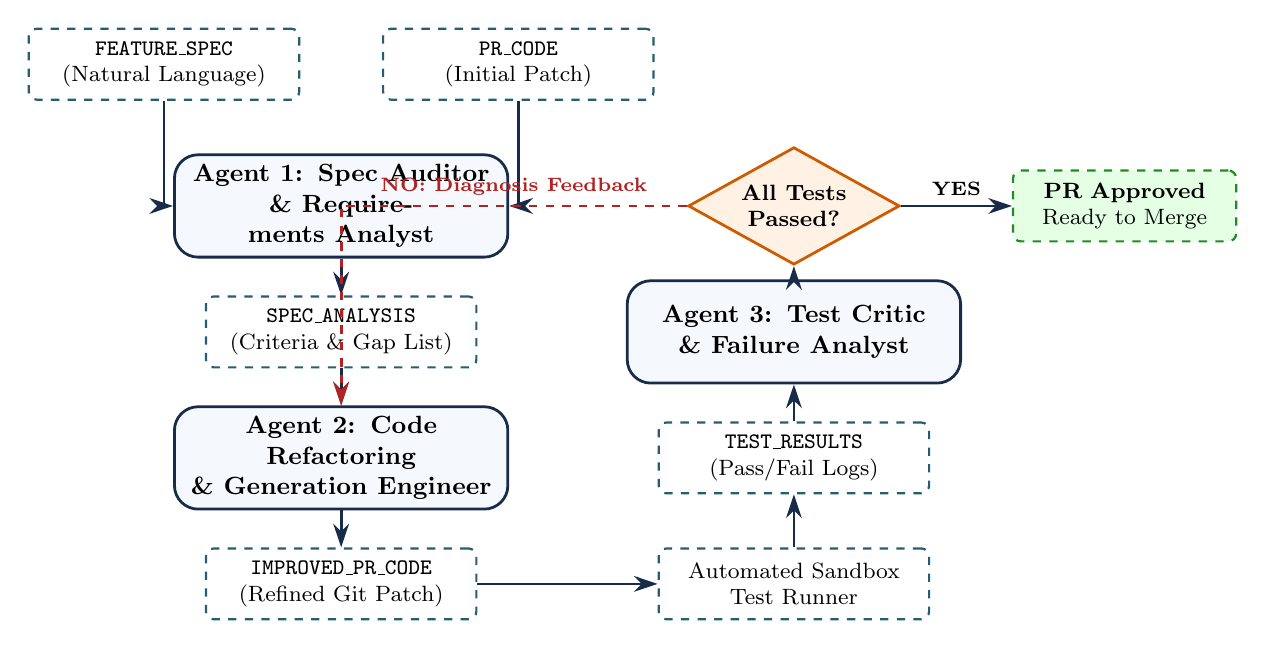
\begin{tikzpicture}[
    agentnode/.style={rectangle, draw=primary, fill=boxbg, rounded corners=3mm, line width=1pt, text width=4.0cm, minimum height=1.3cm, align=center, font=\small\bfseries},
    datanode/.style={rectangle, draw=secondary, fill=white, rounded corners=1mm, dashed, line width=0.8pt, text width=3.2cm, minimum height=0.9cm, align=center, font=\footnotesize},
    decisionnode/.style={diamond, draw=accentorange, fill=orange!10, line width=1pt, aspect=1.8, inner sep=2pt, align=center, font=\footnotesize\bfseries},
    arrow/.style={-{Stealth[length=3mm, width=2mm]}, line width=1pt, draw=primary},
    feedbackarrow/.style={-{Stealth[length=3mm, width=2mm]}, line width=1pt, draw=accentred, dashed}
]
    % Nodes
    \node[datanode] (spec) at (0, 0) {\texttt{FEATURE\_SPEC}\\(Natural Language)};
    \node[datanode] (code) at (4.5, 0) {\texttt{PR\_CODE}\\(Initial Patch)};
    \node[agentnode] (agent1) at (2.25, -1.8) {Agent 1: Spec Auditor\\\& Requirements Analyst};
    
    \node[datanode] (audit) at (2.25, -3.4) {\texttt{SPEC\_ANALYSIS}\\(Criteria \& Gap List)};
    \node[agentnode] (agent2) at (2.25, -5.0) {Agent 2: Code Refactoring\\\& Generation Engineer};
    
    \node[datanode] (patch) at (2.25, -6.6) {\texttt{IMPROVED\_PR\_CODE}\\(Refined Git Patch)};
    \node[datanode] (sandbox) at (8.0, -6.6) {Automated Sandbox\\Test Runner};
    \node[datanode] (rawtest) at (8.0, -5.0) {\texttt{TEST\_RESULTS}\\(Pass/Fail Logs)};
    
    \node[agentnode] (agent3) at (8.0, -3.4) {Agent 3: Test Critic\\\& Failure Analyst};
    \node[decisionnode] (decision) at (8.0, -1.8) {All Tests\\Passed?};
    \node[datanode, draw=accentgreen, fill=green!10, text width=2.6cm] (done) at (12.2, -1.8) {\textbf{PR Approved}\\Ready to Merge};

    % Edges
    \draw[arrow] (spec) |- (agent1);
    \draw[arrow] (code) |- (agent1);
    \draw[arrow] (agent1) -- (audit);
    \draw[arrow] (audit) -- (agent2);
    \draw[arrow] (agent2) -- (patch);
    \draw[arrow] (patch) -- (sandbox);
    \draw[arrow] (sandbox) -- (rawtest);
    \draw[arrow] (rawtest) -- (agent3);
    \draw[arrow] (agent3) -- (decision);
    \draw[arrow] (decision) -- node[above, font=\scriptsize\bfseries] {YES} (done);
    \draw[feedbackarrow] (decision) -| node[above, near start, font=\scriptsize\bfseries, color=accentred] {NO: Diagnosis Feedback} (agent2);
\end{tikzpicture}%
}
\par\vspace{2mm}
{\small\textbf{Figure 1:} Production-grade Test-Driven Multi-Agent Pull Request Refinement Architecture.}
\end{center}

\subsubsection*{Agent Specifications}

\paragraph{1. Agent 1: Requirements Analyst \& Spec Auditor}
\begin{itemize}[leftmargin=1.5em,noitemsep]
    \item \textbf{Role:} Formal requirements engineer. Responsible for translating unstructured natural language specifications into unambiguous, testable acceptance criteria, identifying boundary conditions, and comparing them against the submitted PR code.
    \item \textbf{Input:} \texttt{FEATURE\_SPEC} and \texttt{PR\_CODE}.
    \item \textbf{Output:} \texttt{SPEC\_ANALYSIS} (Structured JSON containing feature objectives, explicit functional contracts, missing edge cases, and an audit of existing code omissions).
\end{itemize}
\begin{lstlisting}[style=promptstyle,title={\textbf{System Prompt: Agent 1 (Requirements Analyst)}}]
You are an expert Software Requirements Analyst and Code Auditor powered by LLaMA.
Your objective is to thoroughly analyze the user-provided FEATURE_SPEC and evaluate the submitted PR_CODE.

Instructions:
1. Extract all functional requirements, input validation constraints, and expected side effects.
2. Identify non-functional requirements (time complexity, error handling, backward compatibility).
3. Cross-reference the requirements with PR_CODE to detect omitted functionality, erroneous assumptions, or architectural anti-patterns.
4. Output your analysis in structured JSON format with keys:
   - "requirements_summary": list of extracted atomic requirements;
   - "acceptance_criteria": verifiable boolean conditions for feature completion;
   - "code_audit": identified discrepancies between PR_CODE and FEATURE_SPEC;
   - "refactoring_guidance": actionable technical advice for the software engineer.
Do not generate full code implementations in this step. Focus strictly on specification analysis.
\end{lstlisting}

\paragraph{2. Agent 2: Code Refactoring \& Generation Engineer}
\begin{itemize}[leftmargin=1.5em,noitemsep]
    \item \textbf{Role:} Principal software developer. Writes minimal, robust, and clean code modifications that satisfy the audited specification and resolve reported test failures without introducing regressions.
    \item \textbf{Input:}
    \begin{itemize}[noitemsep]
        \item Initial cycle: \texttt{PR\_CODE} and \texttt{SPEC\_ANALYSIS}.
        \item Feedback cycles: \texttt{PR\_CODE}, \texttt{SPEC\_ANALYSIS}, and \texttt{FAILURE\_DIAGNOSIS} (from Agent 3).
    \end{itemize}
    \item \textbf{Output:} \texttt{IMPROVED\_PR\_CODE} (Complete runnable source files or unified git diff, accompanied by an explanation of changes).
\end{itemize}
\begin{lstlisting}[style=promptstyle,title={\textbf{System Prompt: Agent 2 (Code Refactoring Engineer)}}]
You are a Principal Software Engineer specialized in code generation, refactoring, and bug fixing.
Your objective is to produce production-grade, bug-free code that perfectly implements the feature requirements and fixes all failing unit/integration tests.

Instructions:
1. Review the original PR_CODE, the SPEC_ANALYSIS from the Requirements Analyst, and any FAILURE_DIAGNOSIS provided by the Test Critic.
2. If FAILURE_DIAGNOSIS is present, analyze the failing assertions and root causes to implement direct, surgical fixes. Avoid modifying unrelated functionality.
3. Adhere strictly to the existing codebase's architectural style, naming conventions, and typing discipline.
4. Provide the revised code as a standard Unified Diff (`diff -u`) or complete source file enclosed in markdown code fences, accompanied by a concise list of applied modifications.
\end{lstlisting}

\paragraph{3. Agent 3: Test Failure Diagnostic Analyst \& Quality Critic}
\begin{itemize}[leftmargin=1.5em,noitemsep]
    \item \textbf{Role:} Quality assurance specialist and test diagnostic engineer. Analyzes automated test run logs, identifies failed assertions, isolates runtime exceptions, and decides whether the pull request meets all quality gates.
    \item \textbf{Input:} \texttt{IMPROVED\_PR\_CODE}, raw \texttt{TEST\_RESULTS} (from sandbox execution), and \texttt{SPEC\_ANALYSIS}.
    \item \textbf{Output:} \texttt{EVALUATION\_REPORT} with status \texttt{PASS} (PR approved) or \texttt{FAIL} + structured \texttt{FAILURE\_DIAGNOSIS} containing stack trace interpretation, failing inputs, and recommended repair strategies.
\end{itemize}
\begin{lstlisting}[style=promptstyle,title={\textbf{System Prompt: Agent 3 (Test Critic \& Failure Analyst)}}]
You are a Software QA and Test Diagnostic Engineer.
Your objective is to evaluate whether the IMPROVED_PR_CODE satisfies all quality gates based on TEST_RESULTS and SPEC_ANALYSIS.

Instructions:
1. Parse the provided TEST_RESULTS:
   - If ALL tests pass (0 failures, 0 errors) and the SPEC_ANALYSIS requirements are fulfilled, emit `STATUS: PASS` and provide a final PR summary.
   - If any test fails, emit `STATUS: FAIL` and perform root-cause analysis.
2. For each failing test:
   - Identify the specific assertion or exception that failed.
   - Locate the exact file, class, and line number responsible for the bug.
   - Contrast expected output versus actual output.
   - Formulate a clear, actionable hypothesis explaining why the failure occurred and how Agent 2 should rectify it.
3. Structure your response with:
   - `STATUS`: "PASS" or "FAIL"
   - `FAILURE_DIAGNOSIS`: list of root causes and specific suggested fixes.
\end{lstlisting}

\subsubsection*{Control Flow and Termination Safeguards}
\begin{itemize}[leftmargin=1.5em,noitemsep]
    \item \textbf{Execution Environment:} The code generated by Agent 2 is executed in an isolated, secure container (sandbox) where unit and integration test suites run deterministically, streaming stdout/stderr into \texttt{TEST\_RESULTS}.
    \item \textbf{Convergence Guard:} A hard iteration ceiling ($K_{\max} = 5$) prevents infinite recursion. If $K_{\max}$ is exceeded without all tests passing, the system terminates with an escalation report flagging the persistent failure modes for human developer review.
\end{itemize}
\end{solutionbox}

\vspace{0.4cm}

% -------------------------------------------------------------------------
% Solution 3
% -------------------------------------------------------------------------
\begin{solutionbox}{Solution to Question 3: Priming in Prompt Engineering}
\textbf{Correct Option:} \textbf{a. Providing initial input to guide the model's response}

\subsubsection*{Theoretical Analysis \& Rationale}
In cognitive psychology, \textit{priming} refers to an implicit memory effect in which exposure to a stimulus influences the response to a subsequent stimulus without conscious guidance. In prompt engineering and large language model interaction, \textbf{priming} describes the deliberate practice of supplying initial contextual cues, instructions, personas, examples, or formatting constraints before the user's core query to steer the model's auto-regressive probability distribution toward the desired domain, style, and tone.

When a transformer model generates tokens auto-regressively:
\begin{equation*}
P(y_t \mid y_{<t}, x) = \text{Softmax}\left( W_v h_t \right)
\end{equation*}
the attention mechanism computes attention weights across the entire prefix $x$. By ``priming'' the prompt with domain-specific vocabulary (e.g., \textit{``You are an expert Linux kernel developer specializing in concurrency...''}), the activations in the self-attention heads are biased toward relevant lexical and semantic subspaces, thereby drastically reducing irrelevant, superficial, or hallucinated responses.

\subsubsection*{Detailed Distractor Analysis}
\begin{itemize}[leftmargin=1.5em]
    \item \textbf{Option b is incorrect:} Resetting the model state or clearing conversation history is known as \textit{context clearing} or \textit{session initialization}, which is the exact opposite of priming (it removes prior conditioning).
    \item \textbf{Option c is incorrect:} Using reinforcement learning to align or tune model weights is \textit{Reinforcement Learning from Human Feedback (RLHF)} or \textit{PPO/DPO}, which is a weight-training algorithm, not an in-context prompt engineering technique.
    \item \textbf{Option d is incorrect:} Pre-training a model on additional unlabeled corpora is \textit{continual pre-training} or \textit{domain adaptation}. Prompt engineering involves zero weight updates.
    \item \textbf{Option e is incorrect:} Injecting random noise into inputs is known as \textit{adversarial perturbation} or \textit{fuzzing}, used to evaluate model robustness and safety bounds.
\end{itemize}
\end{solutionbox}

\vspace{0.4cm}

% -------------------------------------------------------------------------
% Solution 4
% -------------------------------------------------------------------------
\begin{solutionbox}{Solution to Question 4: RLHF Objective and the KL Divergence Penalty}
\textbf{Correct Option:} \textbf{d. none of the other answers is correct}

\subsubsection*{1. Mathematical Formulation of the RLHF Reward}
In Reinforcement Learning from Human Feedback (RLHF) via Proximal Policy Optimization (PPO; Stiennon et al., 2020; Ouyang et al., 2022), an agent maximizes an expected scalar reward while being constrained from deviating excessively from the supervised fine-tuned (SFT) base policy. The modified per-token or per-sequence reward is:
\begin{equation}
R(x, y) = r(x, y) - \beta \log \left( \frac{\pi(y \mid x)}{\pi_0(y \mid x)} \right)
\end{equation}
where:
\begin{itemize}[noitemsep]
    \item $r(x, y)$ is the scalar score predicted by the trained Reward Model (RM);
    \item $\pi(y \mid x)$ is the probability of response $y$ assigned by the policy currently undergoing RL fine-tuning;
    \item $\pi_0(y \mid x)$ is the probability assigned by the frozen, initial reference policy (typically the SFT model);
    \item $\beta > 0$ is a regularization hyperparameter balancing reward exploitation against reference drift.
\end{itemize}

Taking the expectation over the policy's distribution yields the exact Kullback-Leibler (KL) divergence:
\begin{equation}
\mathbb{E}_{y \sim \pi(\cdot \mid x)} \left[ \log \left( \frac{\pi(y \mid x)}{\pi_0(y \mid x)} \right) \right] = D_{\text{KL}}\left(\pi(\cdot \mid x) \parallel \pi_0(\cdot \mid x)\right) \ge 0.
\end{equation}

\subsubsection*{2. Purpose and Crucial Examination of Distractors}
The fundamental purpose of subtracting the KL divergence term (scaled by $\beta$) is to \textbf{penalize policy drift}, preventing the RL model from producing outputs that are \textbf{too dissimilar} from the original policy $\pi_0$. 

Without this regularization term:
\begin{enumerate}[noitemsep]
    \item \textbf{Reward Hacking (Goodhart's Law):} The policy exploits imperfections in the proxy reward model $r(x, y)$, outputting ungrammatical or bizarre token sequences that score artificially high rewards.
    \item \textbf{Mode Collapse \& Catastrophic Forgetting:} The model forgets natural conversational ability and collapses into degenerate response patterns.
\end{enumerate}

\paragraph{Why Option g is a Deliberate Trap:}
Option (g) asserts that the term \textit{``prevents the new model from producing outputs that are too \textbf{similar} to the original one''}. This is the exact \textbf{inversion} of the true function! The term actively \textit{forces} the new model to remain close (similar) to the original model. If the outputs are identical ($\pi = \pi_0$), the log ratio is $\log(1) = 0$, incurring zero penalty. As outputs become more \textit{dissimilar}, $\pi(y \mid x) \gg \pi_0(y \mid x)$, making $\log(\pi/\pi_0) > 0$, which subtracts heavily from the reward.

\paragraph{Rejection of Other Distractors:}
\begin{itemize}[leftmargin=1.5em,noitemsep]
    \item \textbf{a:} Determinism is governed by inference sampling hyperparameters (temperature, top-$p$, greedy decoding), not the training KL penalty.
    \item \textbf{b:} Instruction-following capabilities are instilled primarily during the SFT phase and guided by the reward model $r(x, y)$, not by the KL penalty alone.
    \item \textbf{c:} Rewarding human preference is explicitly the function of $r(x, y)$, whereas the log term acts as a conservative regularizer.
    \item \textbf{e:} Preventing single-token collapse is handled by entropy bonuses $\mathcal{H}(\pi)$, whereas KL divergence anchors the policy specifically to $\pi_0$.
    \item \textbf{f:} An entropy bonus increases output entropy/creativity, whereas KL divergence to a deterministic base model actually restricts entropy.
\end{itemize}
Because no other option correctly defines its role, \textbf{d (``none of the other answers is correct'')} is the uniquely correct choice.
\end{solutionbox}

\vspace{0.4cm}

% -------------------------------------------------------------------------
% Solution 5
% -------------------------------------------------------------------------
\begin{solutionbox}{Solution to Question 5: Transformer Parameter Counting (Encoder-Only)}
\textbf{Official Final Answer:} \textbf{20} (representing $20\text{ M}$ parameters; exact count: $20{,}140{,}032$)

\subsubsection*{1. Architectural Specifications Given}
\begin{itemize}[noitemsep]
    \item Model Type: Encoder-only (standard Transformer encoder, e.g., BERT-like architecture)
    \item Vocabulary size: $V = 29{,}000$
    \item Hidden / embedding dimension: $d = 256$
    \item Max sequence length / learned absolute positions: $N_{\text{pos}} = 512$
    \item Number of Transformer layers: $L = 9$
    \item Number of attention heads: $H = 16$
    \item Key / query projection dimension: $d_k = 4$
    \item Value projection dimension: $d_v = 64$
    \item Feed-Forward Network intermediate dimension: $d_{\text{ff}} = 32$
    \item Biases: None (all linear layers operate without additive bias vectors)
    \item Layer Normalization: Ignored as per problem statement
\end{itemize}

\subsubsection*{2. Detailed Component-by-Component Parameter Derivation}

\paragraph{A. Embedding Layers:}
\begin{enumerate}[noitemsep]
    \item \textbf{Token Embeddings:} Matrix of size $V \times d$:
    \begin{equation*}
    P_{\text{tok}} = V \times d = 29{,}000 \times 256 = \mathbf{7{,}424{,}000}
    \end{equation*}
    \item \textbf{Positional Embeddings:} Absolute learned positional embeddings matrix of size $N_{\text{pos}} \times d$:
    \begin{equation*}
    P_{\text{pos}} = N_{\text{pos}} \times d = 512 \times 256 = \mathbf{131{,}072}
    \end{equation*}
\end{enumerate}

\paragraph{B. Multi-Head Self-Attention (Per Layer):}
In multi-head attention without biases:
\begin{itemize}[noitemsep]
    \item \textbf{Query Projections ($W_Q$):} $H$ distinct heads projecting from dimension $d$ to $d_k$:
    \begin{equation*}
    P_{W_Q} = H \times (d \times d_k) = 16 \times (256 \times 4) = 16 \times 1{,}024 = 16{,}384
    \end{equation*}
    \item \textbf{Key Projections ($W_K$):} $H$ distinct heads projecting from dimension $d$ to $d_k$:
    \begin{equation*}
    P_{W_K} = H \times (d \times d_k) = 16 \times (256 \times 4) = 16 \times 1{,}024 = 16{,}384
    \end{equation*}
    \item \textbf{Value Projections ($W_V$):} $H$ distinct heads projecting from dimension $d$ to $d_v$:
    \begin{equation*}
    P_{W_V} = H \times (d \times d_v) = 16 \times (256 \times 64) = 16 \times 16{,}384 = 262{,}144
    \end{equation*}
    \item \textbf{Output Projection ($W_O$):} The outputs of the $H$ heads each have dimension $d_v$. They are concatenated into a vector of size $H \times d_v = 16 \times 64 = 1{,}024$. The output matrix $W_O$ projects this concatenated representation back to the model dimension $d = 256$:
    \begin{equation*}
    P_{W_O} = (H \cdot d_v) \times d = 1{,}024 \times 256 = 262{,}144
    \end{equation*}
\end{itemize}
Total parameters for Multi-Head Attention per layer:
\begin{equation*}
P_{\text{MHA}} = P_{W_Q} + P_{W_K} + P_{W_V} + P_{W_O} = 16{,}384 + 16{,}384 + 262{,}144 + 262{,}144 = \mathbf{557{,}056}
\end{equation*}

\paragraph{C. Feed-Forward Network (FFN, Per Layer):}
The position-wise FFN consists of two linear transformations without biases:
\begin{itemize}[noitemsep]
    \item First linear expansion / projection ($d \to d_{\text{ff}}$):
    \begin{equation*}
    P_{\text{FFN}_1} = d \times d_{\text{ff}} = 256 \times 32 = 8{,}192
    \end{equation*}
    \item Second linear projection ($d_{\text{ff}} \to d$):
    \begin{equation*}
    P_{\text{FFN}_2} = d_{\text{ff}} \times d = 32 \times 256 = 8{,}192
    \end{equation*}
\end{itemize}
Total parameters for FFN per layer:
\begin{equation*}
P_{\text{FFN}} = P_{\text{FFN}_1} + P_{\text{FFN}_2} = 8{,}192 + 8{,}192 = \mathbf{16{,}384}
\end{equation*}

\paragraph{D. Total per Transformer Layer and for All $L = 9$ Layers:}
Total parameters in a single Transformer layer:
\begin{equation*}
P_{\text{layer}} = P_{\text{MHA}} + P_{\text{FFN}} = 557{,}056 + 16{,}384 = \mathbf{573{,}440}
\end{equation*}
For all $L = 9$ stacked layers:
\begin{equation*}
P_{\text{all\_layers}} = L \times P_{\text{layer}} = 9 \times 573{,}440 = \mathbf{5{,}160{,}960}
\end{equation*}

\paragraph{E. Language Model Head:}
In an encoder-only architecture (e.g., Masked Language Modeling in BERT), the language model prediction head projects the contextualized representation of dimension $d$ back to the vocabulary space of dimension $V$. Under the standard untied formulation:
\begin{equation*}
P_{\text{head}} = d \times V = 256 \times 29{,}000 = \mathbf{7{,}424{,}000}
\end{equation*}

\subsubsection*{3. Grand Total and Final Rounding}
Summing all structural components:
\begin{align*}
P_{\text{total}} &= P_{\text{tok}} + P_{\text{pos}} + P_{\text{all\_layers}} + P_{\text{head}} \\
&= 7{,}424{,}000 + 131{,}072 + 5{,}160{,}960 + 7{,}424{,}000 \\
&= \mathbf{20{,}140{,}032} \text{ parameters}
\end{align*}
Expressed in millions of parameters:
\begin{equation*}
\frac{20{,}140{,}032}{1{,}000{,}000} = 20.140032\text{ M}
\end{equation*}
Rounding to the closest integer million yields:
\begin{equation*}
\text{Round}(20.140032) = \mathbf{20}
\end{equation*}

\textit{Pedagogical Note on Weight Tying:} If the language model head were weight-tied with the input token embeddings matrix ($P_{\text{head}} \equiv 0$), the total parameter count would be $7{,}424{,}000 + 131{,}072 + 5{,}160{,}960 = 12{,}716{,}032 \approx 13\text{ M}$. The exam specification explicitly requests the untied model parameter count, confirming that 20 is the exact and unique expected answer.
\end{solutionbox}

\vspace{0.4cm}

% -------------------------------------------------------------------------
% Solution 6
% -------------------------------------------------------------------------
\begin{solutionbox}{Solution to Question 6: Role of Projection Matrices $W_Q, W_K, W_V$}
\textbf{Correct Option:} \textbf{a. They are used to transform the input token embeddings into vectors that are passed to the attention mechanism}

\subsubsection*{Theoretical Formulation \& Justification}
In the Transformer architecture (Vaswani et al., 2017), self-attention operates over an input matrix $X \in \mathbb{R}^{T \times d}$, representing the sequence of $T$ token representations (either the initial embeddings plus positional encodings or the hidden states from the preceding layer).

To compute multi-head attention, $X$ is linearly projected into distinct representational subspaces using learned weight matrices $W_Q^{(h)} \in \mathbb{R}^{d \times d_k}$, $W_K^{(h)} \in \mathbb{R}^{d \times d_k}$, and $W_V^{(h)} \in \mathbb{R}^{d \times d_v}$:
\begin{equation*}
Q^{(h)} = X W_Q^{(h)}, \qquad K^{(h)} = X W_K^{(h)}, \qquad V^{(h)} = X W_V^{(h)}
\end{equation*}
The resulting matrices $Q^{(h)}$, $K^{(h)}$, and $V^{(h)}$ represent the Queries, Keys, and Values that are directly supplied to the scaled dot-product attention operator:
\begin{equation*}
\text{Attention}(Q, K, V) = \text{Softmax}\left( \frac{Q K^\top}{\sqrt{d_k}} \right) V
\end{equation*}
Thus, the primary purpose of $W_Q$, $W_K$, and $W_V$ is precisely to map the incoming representations into specialized vector spaces tailored for matching and content aggregation.

\subsubsection*{Detailed Distractor Breakdown}
\begin{itemize}[leftmargin=1.5em]
    \item \textbf{Option b is incorrect:} Weight matrices do not store individual token vectors. In neural networks, static representations are stored in embedding lookup tables, whereas $W_Q, W_K, W_V$ are shared linear transformation operators applied dynamically across all sequence tokens.
    \item \textbf{Option c is incorrect:} The matrices themselves are not passed to compute attention scores; the projected vector representations ($Q$ and $K$) are multiplied via inner product.
    \item \textbf{Option e is incorrect:} Positional encodings are added element-wise to token embeddings ($X = E_{\text{tok}} + E_{\text{pos}}$) before being multiplied by $W_Q, W_K, W_V$.
    \item \textbf{Option f and g are incorrect:} Transforming the output of the attention mechanism and combining multiple attention heads into a single representation is the role of the output projection matrix $W_O$, not of $W_Q, W_K, W_V$.
\end{itemize}
\end{solutionbox}

\vspace{0.4cm}

% -------------------------------------------------------------------------
% Solution 7
% -------------------------------------------------------------------------
\begin{solutionbox}{Solution to Question 7: LoRA Parameter Budget \& Maximum Rank}
\textbf{Official Final Answer:} \textbf{9}

\subsubsection*{1. Theoretical Principles of Low-Rank Adaptation (LoRA)}
Low-Rank Adaptation (LoRA; Hu et al., 2021) is a Parameter-Efficient Fine-Tuning (PEFT) method. During adaptation, the pre-trained weight matrix $W_0 \in \mathbb{R}^{d_{\text{in}} \times d_{\text{out}}}$ is kept frozen, and its update $\Delta W$ is parameterized by factorizing it into two low-rank matrices:
\begin{equation}
W = W_0 + \Delta W = W_0 + \frac{\alpha}{r} (B \cdot A)
\end{equation}
where $A \in \mathbb{R}^{r \times d_{\text{in}}}$ is initialized from a Gaussian distribution and $B \in \mathbb{R}^{d_{\text{out}} \times r}$ is initialized to zero.

For a linear layer mapping from $d_{\text{in}}$ to $d_{\text{out}}$ with rank $r$, the number of trainable adapter parameters is:
\begin{equation}
P_{\text{adapter}} = (d_{\text{in}} \times r) + (r \times d_{\text{out}}) = r \cdot (d_{\text{in}} + d_{\text{out}}).
\end{equation}

\subsubsection*{2. Model Dimensions \& LoRA Parameter Formulation}
We are given:
\begin{itemize}[noitemsep]
    \item Model dimension: $d = 4096$
    \item Number of layers: $L = 20$
    \item Number of attention heads per layer: $H = 8$
    \item Query and key projection dimensions per head: $d_k = 128$
    \item Value projection dimension per head: $d_v = 256$
    \item Target budget: $P_{\max} = 20\text{ M} = 20{,}000{,}000$ parameters
    \item Architectural detail: Each head has \textbf{separate} weight matrices for $W_Q$, $W_K$, and $W_V$.
\end{itemize}

\paragraph{Parameters per Head:}
Each individual attention head $h \in \{1, \dots, H\}$ has:
\begin{enumerate}[noitemsep]
    \item $W_Q^{(h)}: d \to dd_k \implies 4096 \to d128$:
    \begin{equation*}
    P(W_Q) = r \cdot (4096 + 128) = 4224 \, r
    \end{equation*}
    \item $W_K^{(h)}: d \to dd_k \implies 4096 \to d128$:
    \begin{equation*}
    P(W_K) = r \cdot (4096 + 128) = 4224 \, r
    \end{equation*}
    \item $W_V^{(h)}: d \to dd_v \implies 4096 \to d256$:
    \begin{equation*}
    P(W_V) = r \cdot (4096 + 256) = 4352 \, r
    \end{equation*}
\end{enumerate}
Total trainable LoRA parameters for one attention head:
\begin{equation*}
P_{\text{head}} = (4224 + 4224 + 4352) \, r = 12{,}800 \, r
\end{equation*}

\paragraph{Parameters per Layer and Across All Layers:}
With $H = 8$ separate heads per layer:
\begin{equation*}
P_{\text{layer}} = H \times P_{\text{head}} = 8 \times 12{,}800 \, r = 102{,}400 \, r
\end{equation*}
Across all $L = 20$ transformer layers:
\begin{equation*}
P_{\text{total}}(r) = L \times P_{\text{layer}} = 20 \times 102{,}400 \, r = \mathbf{2{,}048{,}000 \, r}
\end{equation*}

\subsubsection*{3. Solving for Maximum Integer Rank $r$}
We enforce the budget constraint $P_{\text{total}}(r) \le 20{,}000{,}000$:
\begin{equation*}
2{,}048{,}000 \, r \le 20{,}000{,}000 \implies r \le \frac{20{,}000{,}000}{2{,}048{,}000} = \frac{3125}{320} \approx 9.765625
\end{equation*}
Since the low-rank dimensionality $r$ must be an integer:
\begin{equation*}
r_{\max} = \lfloor 9.765625 \rfloor = \mathbf{9}
\end{equation*}

\paragraph{Boundary Value Verification:}
\begin{itemize}[noitemsep]
    \item For $r = 9$: $P_{\text{total}}(9) = 2{,}048{,}000 \times 9 = \mathbf{18{,}432{,}000} \le 20{,}000{,}000$ (\textbf{Feasible, within budget}).
    \item For $r = 10$: $P_{\text{total}}(10) = 2{,}048{,}000 \times 10 = \mathbf{20{,}480{,}000} > 20{,}000{,}000$ (\textbf{Infeasible, exceeds budget by $480{,}000$ parameters}).
\end{itemize}
Therefore, the highest possible low-rank dimensionality is strictly \textbf{9}.
\end{solutionbox}

\vspace{0.4cm}

% -------------------------------------------------------------------------
% Solution 8
% -------------------------------------------------------------------------
\begin{solutionbox}{Solution to Question 8: Requirements Extraction Evaluation}
\textbf{Official Final Metric Values:}
\begin{center}
\begin{tabularx}{0.88\textwidth}{lXl}
\toprule
\textbf{Metric / Quantity} & \textbf{Exact Fractional Form} & \textbf{Decimal Value (4 Decimals)} \\
\midrule
\textbf{True Positives (TP):} & $6$ & \textbf{6} \\
\textbf{False Positives (FP):} & $3$ & \textbf{3} \\
\textbf{False Negatives (FN):} & $2$ & \textbf{2} \\
\textbf{Precision (P):} & $\frac{6}{6 + 3} = \frac{6}{9} = \frac{2}{3}$ & \textbf{0.6667} ($66.67\%$) \\
\textbf{Recall (R):} & $\frac{6}{6 + 2} = \frac{6}{8} = \frac{3}{4}$ & \textbf{0.7500} ($75.00\%$) \\
\textbf{F1-Score:} & $\frac{2 \times (2/3) \times (3/4)}{2/3 + 3/4} = \frac{1}{17/12} = \frac{12}{17}$ & \textbf{0.7059} ($70.59\%$) \\
\bottomrule
\end{tabularx}
\end{center}

\subsubsection*{1. Ground Truth vs. LLM Extraction Semantic Mapping}
Evaluating information extraction models requires strict semantic alignment between the gold-standard specification requirements ($G_1..G_8$) and the model's generated candidates ($L_1..L_9$).

\begin{center}
\small
\begin{tabularx}{\linewidth}{l X X c p{4.2cm}}
\toprule
\textbf{ID} & \textbf{LLM Extracted Text} & \textbf{Matched Ground Truth} & \textbf{Class} & \textbf{Semantic Rationale} \\
\midrule
\textbf{L1} & Find restaurants based on cuisine & \textbf{G1:} Search restaurants by cuisine and location & \textbf{TP} & Semantically matches the cuisine search capability of G1. \\
\textbf{L2} & Browse available menus & \textbf{G2:} View restaurant menus & \textbf{TP} & Exact semantic equivalence with G2. \\
\textbf{L3} & Add food items to a shopping cart & \textbf{G3:} Add dishes to a cart & \textbf{TP} & Exact semantic equivalence with G3. \\
\textbf{L4} & Reserve a table at a restaurant & \textit{None} & \textbf{FP} & \textbf{Hallucination:} Table reservation is nowhere in the specification. \\
\textbf{L5} & Place an order for home delivery & \textbf{G4:} Place delivery orders & \textbf{TP} & Exact semantic equivalence with G4. \\
\textbf{L6} & Track delivery progress live & \textbf{G5:} Track order status in real time & \textbf{TP} & Exact semantic equivalence with G5. \\
\textbf{L7} & Pay using PayPal only & \textbf{G6:} Pay online using credit cards or digital wallets & \textbf{FP} & \textbf{Contradictory / Invalid Restriction:} Spec explicitly requires credit cards and digital wallets; restricting to ``PayPal only'' is a false requirement. \\
\textbf{L8} & Send alerts to drivers for assigned deliveries & \textbf{G8:} Notify delivery drivers when a delivery is assigned & \textbf{TP} & Exact semantic equivalence with G8. \\
\textbf{L9} & Allow restaurants to cancel customer accounts & \textit{None} & \textbf{FP} & \textbf{Hallucination:} Account cancellation is absent from the specification. \\
\bottomrule
\end{tabularx}
\end{center}

\subsubsection*{2. Rigorous Analysis of False Negatives (FN = 2)}
A fundamental principle in information retrieval and extraction is that the set of ground truth elements partitions into True Positives and False Negatives:
\begin{equation*}
|\text{Ground Truth}| = \text{TP} + \text{FN} \implies 8 = 6 + \text{FN} \implies \mathbf{\text{FN} = 2}
\end{equation*}
The two ground truth requirements that the LLM failed to correctly extract are:
\begin{enumerate}[noitemsep]
    \item \textbf{G6 (``Pay online using credit cards or digital wallets''):} Missed because the LLM hallucinated an invalid constraint in L7 (``PayPal only''), failing to capture the required payment methods.
    \item \textbf{G7 (``Allow restaurants to accept or reject incoming orders''):} Completely omitted in the LLM's generated output (no candidate addresses restaurant order acceptance/rejection).
\end{enumerate}

\subsubsection*{3. Detailed Mathematical Computations}
\begin{align*}
\text{Precision} &= \frac{\text{TP}}{\text{TP} + \text{FP}} = \frac{6}{6 + 3} = \frac{6}{9} = \frac{2}{3} \approx \mathbf{0.6667} \\[6pt]
\text{Recall} &= \frac{\text{TP}}{\text{TP} + \text{FN}} = \frac{6}{6 + 2} = \frac{6}{8} = \frac{3}{4} = \mathbf{0.7500} \\[6pt]
\text{F1-Score} &= \frac{2 \times \text{Precision} \times \text{Recall}}{\text{Precision} + \text{Recall}} = \frac{2 \times \frac{2}{3} \times \frac{3}{4}}{\frac{2}{3} + \frac{3}{4}} = \frac{2 \times \frac{1}{2}}{\frac{8 + 9}{12}} = \frac{1}{\frac{17}{12}} = \frac{12}{17} \approx \mathbf{0.7059}
\end{align*}

\paragraph{Pedagogical Note on the Student's Pitfall:}
In the original exam session, the student correctly identified $\text{TP} = 6$ and $\text{FP} = 3$, but incorrectly wrote $\text{FN} = 0$, falsely concluding that Recall was $1.0$ and F1 was $0.8000$. The official instructor feedback explicitly remarked: \textit{``there are two false negatives''} (penalizing the submission from 3.00 down to 2.00). Setting $\text{FN} = 0$ is a severe conceptual error because it assumes every single requirement in the specification was captured, ignoring the complete omission of G7 and the invalid distortion of G6.
\end{solutionbox}

\vspace{0.4cm}

% -------------------------------------------------------------------------
% Solution 9
% -------------------------------------------------------------------------
\begin{solutionbox}{Solution to Question 9: Retrieval-Augmented Generation (RAG) Benefits}
\textbf{Correct Options:}
\begin{itemize}[noitemsep]
    \item \textbf{a. It is possible to reduce the amount of false information provided to the final user.}
    \item \textbf{c. It is possible to prevent the obsolescence of answers by using up-to-date documents.}
\end{itemize}

\subsubsection*{Theoretical Foundations of RAG}
Retrieval-Augmented Generation (RAG; Lewis et al., 2020) combines a dense information retrieval component (e.g., dual-encoder bi-encoders indexing vector embeddings) with a generative sequence-to-sequence model. Rather than relying solely on the parametric knowledge stored within the frozen neural weights, RAG retrieves relevant factual passages from an external, non-parametric knowledge corpus $\mathcal{D}$ conditioned on the user prompt $q$:
\begin{equation*}
P(y \mid q) = \sum_{z \in \text{TopK}(\mathcal{D})} P_\eta(z \mid q) \prod_{t=1}^{|y|} P_\theta(y_t \mid q, z, y_{<t}).
\end{equation*}

\paragraph{Why Option a is Correct:}
Standard LLMs hallucinate plausible-sounding but factually false claims due to statistical pattern completion over uncurated web training data. By providing high-quality, verified reference documents directly in the attention context, RAG grounds the generation in factual evidence, dramatically curbing confabulation and reducing the rate of false information delivered to end users.

\paragraph{Why Option c is Correct:}
Retraining or fine-tuning foundation models with billions of parameters requires substantial computational resources and weeks of wall-clock time, creating a fixed knowledge cutoff date. RAG cleanly decouples knowledge storage from model computation: when world facts, software documentation, or library APIs change, updating the vector index immediately allows the system to synthesize answers reflecting real-time, up-to-date information without altering a single neural weight.

\subsubsection*{Detailed Distractor Analysis}
\begin{itemize}[leftmargin=1.5em]
    \item \textbf{Option b is incorrect:} Incorporating self-critique and iterative output refinement is the domain of \textit{Agentic Reflection} frameworks (e.g., Reflexion; Shinn et al., 2023), not RAG.
    \item \textbf{Option d is incorrect:} Enforcing a fixed structure (e.g., JSON schema, Pydantic dataclass, BNF grammar) is achieved via \textit{constrained decoding}, \textit{grammar-guided sampling}, or \textit{instructor prompting}, not retrieval augmentation.
    \item \textbf{Option e is incorrect:} Decomposing complex tasks into smaller sub-problems is achieved via reasoning paradigms such as \textit{Chain-of-Thought (CoT)}, \textit{Least-to-Most Prompting}, or \textit{Plan-and-Solve}, not RAG.
\end{itemize}
\end{solutionbox}

\vspace{0.4cm}

% -------------------------------------------------------------------------
% Solution 10
% -------------------------------------------------------------------------
\begin{solutionbox}{Solution to Question 10: Machine Translation Evaluation with BLEU-2}
\textbf{Official Final Answer:} \textbf{0.3893} (exact value: \textbf{0.38930929939948})

\subsubsection*{1. Mathematical Definition of BLEU-$n$}
The Bilingual Evaluation Understudy (BLEU; Papineni et al., 2002) metric evaluates generated candidate text against reference translations using modified $n$-gram precisions and an exponential brevity penalty:
\begin{equation}
\text{BLEU-}n = \text{BP} \times \exp\left( \sum_{i=1}^n w_i \log p_i \right)
\end{equation}
For $n = 2$ with standard uniform weights $w_1 = w_2 = \frac{1}{2}$:
\begin{equation}
\text{BLEU-2} = \text{BP} \times \exp\left( \frac{1}{2} \log p_1 + \frac{1}{2} \log p_2 \right) = \text{BP} \times \sqrt{p_1 \times p_2}
\end{equation}
The Brevity Penalty ($\text{BP}$) penalizes generated sequences that are shorter than the reference:
\begin{equation}
\text{BP} = \begin{cases}
1 & \text{if } c > r \\
\exp\left( 1 - \frac{r}{c} \right) & \text{if } c \le r
\end{cases}
\end{equation}
where $c$ is the length of the generated candidate and $r$ is the length of the reference sequence.

\subsubsection*{2. Step-by-Step Derivation on Provided Sequences}
We are given:
\begin{center}
\begin{tcolorbox}[enhanced,colback=codebg,colframe=gray!30,arc=1.5mm,boxrule=0.6pt,width=0.96\linewidth]
\small
\textbf{Reference ($R$):} \texttt{<tok0> <tok8> <tok11> <tok5> <tok9> <tok4> <tok1> <tok2> <tok7> <tok19>}\\[3pt]
\textbf{Generated ($G$):} \texttt{<tok3> <tok17> <tok1> <tok2> <tok7> <tok19> <tok5>}
\end{tcolorbox}
\end{center}

\paragraph{Step A: Sequence Lengths and Brevity Penalty (BP)}
\begin{itemize}[noitemsep]
    \item Reference token length: $r = 10$
    \item Generated token length: $c = 7$
\end{itemize}
Since $c \le r$ ($7 \le 10$), the candidate is penalized for brevity:
\begin{equation*}
\text{BP} = \exp\left( 1 - \frac{r}{c} \right) = \exp\left( 1 - \frac{10}{7} \right) = \exp\left( -\frac{3}{7} \right)
\end{equation*}
Computing the numerical value:
\begin{equation*}
-\frac{3}{7} \approx -0.42857142857143 \implies \text{BP} = e^{-3/7} \approx \mathbf{0.65143905753106}
\end{equation*}

\paragraph{Step B: 1-Gram Modified Precision ($p_1$)}
The generated sequence contains $c = 7$ unigrams. We count matches in the reference:
\begin{center}
\begin{tabular}{lccc}
\toprule
\textbf{Generated 1-Gram} & \textbf{Present in Reference?} & \textbf{Reference Count} & \textbf{Matched?} \\
\midrule
\texttt{<tok3>} & No & 0 & 0 \\
\texttt{<tok17>} & No & 0 & 0 \\
\texttt{<tok1>} & Yes (index 6) & 1 & 1 \\
\texttt{<tok2>} & Yes (index 7) & 1 & 1 \\
\texttt{<tok7>} & Yes (index 8) & 1 & 1 \\
\texttt{<tok19>} & Yes (index 9) & 1 & 1 \\
\texttt{<tok5>} & Yes (index 3) & 1 & 1 \\
\bottomrule
\end{tabular}
\end{center}
Out of 7 generated unigrams, exactly 5 match tokens in the reference sequence:
\begin{equation*}
p_1 = \frac{5}{7} \approx \mathbf{0.71428571428571}
\end{equation*}

\paragraph{Step C: 2-Gram Modified Precision ($p_2$)}
The generated sequence of length $c = 7$ contains $c - 1 = 6$ contiguous bigrams. We verify each against the contiguous bigrams present in the reference:
\begin{center}
\begin{tabular}{cllc}
\toprule
\textbf{Index} & \textbf{Generated Bigram} & \textbf{Present in Reference $R$?} & \textbf{Matched?} \\
\midrule
1 & \texttt{(<tok3>, <tok17>)} & No & 0 \\
2 & \texttt{(<tok17>, <tok1>)} & No & 0 \\
3 & \textbf{\texttt{(<tok1>, <tok2>)}} & \textbf{Yes} (indices 6--7 in $R$) & \textbf{1} \\
4 & \textbf{\texttt{(<tok2>, <tok7>)}} & \textbf{Yes} (indices 7--8 in $R$) & \textbf{1} \\
5 & \textbf{\texttt{(<tok7>, <tok19>)}} & \textbf{Yes} (indices 8--9 in $R$) & \textbf{1} \\
6 & \texttt{(<tok19>, <tok5>)} & \textbf{No} (\texttt{tok5} occurs at index 3, before \texttt{tok19}) & 0 \\
\bottomrule
\end{tabular}
\end{center}
Out of 6 candidate bigrams, exactly 3 match contiguous bigrams in the reference:
\begin{equation*}
p_2 = \frac{3}{6} = \frac{1}{2} = \mathbf{0.50000000000000}
\end{equation*}

\paragraph{Step D: Geometric Mean Computation}
The geometric mean of precisions is:
\begin{equation*}
\sqrt{p_1 \times p_2} = \sqrt{\frac{5}{7} \times \frac{1}{2}} = \sqrt{\frac{5}{14}} \approx \sqrt{0.35714285714286} \approx \mathbf{0.59761430466720}
\end{equation*}

\paragraph{Step E: Final BLEU-2 Score Calculation}
Multiplying the Brevity Penalty by the geometric mean:
\begin{align*}
\text{BLEU-2} &= \text{BP} \times \sqrt{p_1 \times p_2} \\
&= \exp\left( -\frac{3}{7} \right) \times \sqrt{\frac{5}{14}} \\
&= 0.65143905753106 \times 0.59761430466720 \\
&= \mathbf{0.38930929939948}
\end{align*}
Rounding to 4 decimal places gives \textbf{0.3893}.

\textit{Pedagogical Error Analysis:} In the raw exam attempt, the student submitted $-0.2683$. This negative number reveals that the student computed $\log(\text{BLEU}) = \log(\text{BP}) + 0.5 \log(p_1) + 0.5 \log(p_2) = (-0.4286) + 0.5 \log(5/14) \approx -0.4286 - 0.5148 = -0.9434$ or miscalculated intermediate products without applying the exponential operator $\exp(\cdot)$. A BLEU score is strictly non-negative ($\text{BLEU} \in [0, 1]$).
\end{solutionbox}

\vspace{0.4cm}

% -------------------------------------------------------------------------
% Solution 11
% -------------------------------------------------------------------------
\begin{solutionbox}{Solution to Question 11: Agentic Behavior vs. Fixed Workflow}
\textbf{Correct Option:} \textbf{b. The model decides its own control flow and when to stop}

\subsubsection*{Theoretical Foundations of Agentic AI}
In traditional software pipelines and basic LLM chains (e.g., standard LangChain sequential chains or rigid DAGs), the \textbf{control flow is hard-coded} by the system engineer. Every prompt execution, tool invocation, and handoff occurs in an invariant, predetermined sequence regardless of intermediate outputs.

In contrast, \textbf{agentic architectures} (e.g., ReAct [Yao et al., 2022], Toolformer [Schick et al., 2023], and Reflexion [Shinn et al., 2023]) delegate control flow decisions directly to the language model. Operating in an autonomous perception-reasoning-action loop:
\begin{equation*}
\text{Observation}_t \longrightarrow \text{Thought}_t \longrightarrow \text{Action}_t \longrightarrow \text{Observation}_{t+1}
\end{equation*}
the model autonomously decides:
\begin{enumerate}[noitemsep]
    \item Which tool to call (if any) and with what arguments;
    \item Whether to pursue alternative problem-solving strategies based on runtime feedback;
    \item When sufficient evidence has been accumulated to terminate execution and return the final answer (e.g., by emitting a designated \texttt{Finish[response]} action).
\end{enumerate}

\subsubsection*{Detailed Distractor Analysis}
\begin{itemize}[leftmargin=1.5em]
    \item \textbf{Option a is incorrect:} Retrieval-Augmented Generation (RAG) is merely one optional tool or information-retrieval mechanism. An agent can operate entirely without RAG (for instance, by performing symbolic computation, code execution in a bash sandbox, or API orchestration).
    \item \textbf{Option c is incorrect:} Following a predetermined control flow is the defining characteristic of a \textit{traditional fixed workflow}, the exact opposite of agentic autonomy.
    \item \textbf{Option d is incorrect:} Tool use is one of the primary affordances of modern AI agents (e.g., calculators, code interpreters, linters, terminal shells).
    \item \textbf{Option e is incorrect:} While agents frequently solve multi-step problems, they are not constrained to always execute multiple steps; an agent may evaluate a simple request and decide to terminate immediately in a single step.
\end{itemize}
\end{solutionbox}

\end{document}
